\section{Generalized unitarity}\label{sect-unitarity}
Bern, Dixon, Dunbar and Kosower proposed a procedure~\cite{Bern:1994zx} based on the Cutkosky rules~\cite{doi:10.1063/1.1703676} which allows to determine compute amplitudes in a gauge field theory in a more efficient way than the traditional diagrammatic methods. 
Especially, in their paper~\cite{Bern:1994zx}, they showed how the generalized unitarity can be applied to the N=4 super Yang-Mills theory thanks to the fact that only scalar box integrals involve in amplitudes after reduction.
\\\\
Based on Landau's discussion on the singularities of the amplitudes calculated from an arbitrary Feynman diagram~\cite{LANDAU1959181}, 
Cutkosky proposed a generalized version of the unitarity condition~\cite{doi:10.1063/1.1703676} which is based on the discontinuity across a cut starting from any of Landau's branch points.
\\
The simplest physical cut is a double cut (or a two-particle cut).
Let us consider a generic one-loop amplitude with explicit dependence on the kinematic invariant $K^2$
\begin{equation*}
A(K^2) = \int\frac{\dd^D l}{(2\pi)^D} A_L\frac{1}{l^{2} (l-K)^{2}}A_R
\end{equation*}
where $A_{L,R}$ are rational fractions in the loop momentum $l$ and the external momenta. 
In Cutkosky's language, a double cut amounts to choose two of the propagators in the loop on-shell.
Mathematically, this means doing the following propagator subsitutions\footnote{One should be careful with the $i\epsilon$ prescription which is often omitted in amplitude computations}
\begin{equation}\label{on-shell_propagator}
\frac{1}{l^2 + i\epsilon} \rightarrow 2\pi i\delta^{(+)}\big(l^2\big)
\quad,\quad
\frac{1}{(l-K)^2 + i\epsilon} \rightarrow 2\pi i\delta^{(+)}\big((l-K)^2\big)
\end{equation}
We call this a double cut in the $K^2$-channel.
Cutkosky's rules states that we will get the branch cut, \ie the discontinuity of $A$ between approching the branch $K^2$ from above and approching from below on the complex plan
\begin{equation}\label{cutkosky}
A(K^2 + i\epsilon) - A(K^2 - i\epsilon) =
-4\pi^2 \int\frac{\dd^D l}{(2\pi)^D}A^{\mathrm{tree}}_LA^{\mathrm{tree}}_R \delta^{(+)}(l^2)\delta^{(+)}\big((l-K)^2\big) 
\end{equation}
Here, $A_L$ and $A_R$ become genuine amplitudes at tree-level because of the on-shell internal propagators. 
\\\\
We illustrate~\cref{cutkosky} by two different examples.
%
%
\begin{figure}[h]
  \centering
  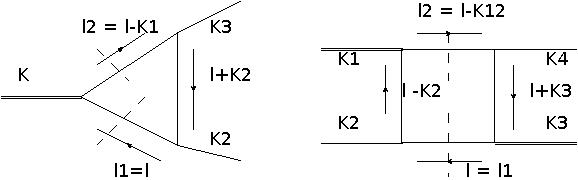
\includegraphics[width=0.8\linewidth]{cutkosky.jpg}
  \caption{One-mass triangle and two-mass-easy box integrals and their cuts}
  \label{fig-cutkosky}
\end{figure}
\subsection{Example: cut one-mass triangle}
%\section{1m triangle cut}
Let us first consider the one-mass triangle integral with massive external leg $K^2 \neq 0$ (left of~\ref{fig-cutkosky})
\begin{equation*}
I_3 = \int\frac{\dd^D l }{(2\pi)^D}\frac{1}{l^2(l-K)^2(l+K_2)^2}
\end{equation*}
As mentioned earlier, we use the dimensional regularization scheme with $D = 4-2\epsilon$.
This integral can be computed using the standard techniques: Feynman parametrization and Wick rotation (since the integrant vanishes at infinity)
\begin{equation*}
\begin{split}
I_3 = & \int\frac{\dd^D l }{(2\pi)^D}\int_0^{1} \dd x \int_0^{1-x}\dd y \frac{2!}{(l^2 - x^2 K^2 + xK^2 + 2xy K\cdot K_2)^3}
\\
= &
-\frac{i}{(4\pi)^{2-\epsilon}}\Gamma (1+\epsilon)
\int^1_0 \dd x\int_0^1 \dd u x^{-1-\epsilon} (1-x)^{-1-\epsilon}
\frac{1}{(-K^2 - 2uK\cdot K_2)^{1+\epsilon}}
\\
= &
\frac{i}{(4\pi)^{2-\epsilon}}\frac{\Gamma^2(1-\epsilon)\Gamma(1+\epsilon)}{\Gamma(1-2\epsilon)}
\frac{1}{\epsilon^2}(-K^2)^{-1-\epsilon}
\end{split}
\end{equation*}
where a change of variable $u =\frac{1}{(1-x)}y$ is used in the second line and $K_3^2 = 0$ is used to obtain the final result.
\\
Now, let us do a cut on the $K_1^2$-channel. 
The uncut internal leg carries momentum $l + K_2$. 
We choose to work in the center-of-mass frame of the massive leg.
%
\begin{equation*}
\begin{split}
\Delta I_3^{1m} = \int\dd \Pi_{\textrm{LIPS}}(l, l-K) \frac{1}{(l+K_2)^2} & =
\int\frac{\dd^{D-1}l_1}{(2\pi)^{D-1}}\int\frac{\dd^{D-1}l_2}{(2\pi)^{D-1}}
\frac{(2\pi)^{D}\delta^{D}(l_1 + l_2 - K)}{8(l\cdot K_2)l_1^0 l_2^0}
\\
& = \int\frac{\dd^{D-1}l_1}{(2\pi)^{D-2}}\frac{\delta(l_1^0 + l_2^0 - K^0)}{2(l\cdot K_2)(K^0)^2} 
\\
& = \int\frac{|\vec{l}|^{D-2}\dd |\vec{l}|}{(2\pi)^{D-2}} \frac{\dd\Omega_{D-1}\delta(l_1^0 + l_2^0 - K^0)}{2 ( l \cdot K_2)(K^0)^2}
\\
& = \frac{1}{2}\frac{\Omega_{D-2}\big(\frac{K^0}{2}\big)^{D-2}}{(2\pi)^{D-2}(K_0)^3 K^0_2} \int_{-1}^1\dd z (1-z)^{-1-\epsilon}(1+z)^{-\epsilon}
\end{split} 
\end{equation*}
The factor of $\frac{1}{2}$ in the last line comes from the delta function in the second last line.
%
The last integral gives a beta-function
%
\begin{equation*}
\begin{split}
\int^1_{-1} (1-z)^{-1-\epsilon}(1+z)^{-\epsilon} \dd z 
=\int^1_0(2s)^{-\epsilon} 2^{-1-\epsilon} (1-s)^{-1-\epsilon} 2 \dd s
=2^{-2\epsilon}\frac{\Gamma(-\epsilon)\Gamma(1-\epsilon)}{\Gamma(1-2\epsilon)}
\end{split}
\end{equation*}
%
As a result, the cut in terms of the invariants is
\begin{equation*}
\Delta I_3^{1m} = 
\frac{2\pi^{\frac{D}{2}-1}}{\Gamma(\frac{D}{2}-1)}\frac{\big(\frac{K^2}{4}\big)^{\frac{D-2}{2}}}{(2\pi)^{D-2}K^2(K_2\cdot K)} 2^{-2\epsilon}\frac{\Gamma(-\epsilon)\Gamma(1-\epsilon)}{\Gamma(1-2\epsilon)}
=
-\frac{1}{(4\pi)^{1 - \epsilon}\epsilon}(K^{2})^{-1-\epsilon}\frac{\Gamma(1-\epsilon)}{\Gamma(1-2\epsilon)}
\end{equation*}
We verify that, up to the order of $\mathcal{O}(\epsilon^{-1})$, this corresponds to the branch cut of $I_3$ across the branch $K^2 > 0$.
\subsection{Example: cut two-mass-easy box}
The easy-two-mass box integral has two opposite massive external legs (cf. right of figure~\ref{fig-cutkosky}).
Using a Feynman parametrization, the 2-mass easy box integral with massless internal lines in $D=4-2\epsilon$ dimension corresponds to the integral \begin{equation}
\begin{split}
I_4 & = \int\frac{\dd^D l }{(2\pi)^D}\frac{1}{ l^2(l-K_1)^2(l+K_4)^2 (l-K_{12}^2)}
\\
&=
3!\times\int\frac{\dd^D l }{(2\pi)^D}
\int
\frac{\prod_{i=1}^4\dd\alpha_i \delta(\sum_{i=1}^4\alpha_i -1)}{\big[\alpha_1(l-K_1)^2 + \alpha_2(l+K_4)^2 + \alpha_3 (l-K_{12}^2) + \alpha_4\big]^4}
\\
&= \frac{i\Gamma(2+\epsilon)}{(4\pi)^{2-\epsilon}}\int\prod_{i=1}^4\dd\alpha_i \delta(\sum_{i=1}^4\alpha_i -1)\frac{1}{(-\alpha_1\alpha_2 t - \alpha_3\alpha_4 s 
-\alpha_1\alpha_4 K_1^2 - \alpha_2\alpha_3 K_{3}^2)^{2+\epsilon}}
\end{split}
\end{equation}
where
\begin{equation}
s=K_{12}^2 \quad\mathrm{and}\quad t=K_{14}^2
\end{equation}
Using the following change of variables
\begin{equation}
\alpha_1 = xy \quad,\quad
\alpha_2 = z(1-y)\quad,\quad
\alpha_3 = y(1-x)\quad,\quad
\alpha_4 = (1-y)(1-z)
\end{equation}
the above integral can be written as
\begin{equation}
I_4 = \frac{i\Gamma(2+\epsilon)}{(4\pi)^{2-\epsilon}} I
\end{equation}
where
\begin{equation}\label{box_int_I}
I = \int\dd x\dd y \dd z y^{-1-\epsilon}(1-y)^{-1-\epsilon}s^{-2-\epsilon}
\frac{1}{(-1 + A_1 x + A_3 z + C xz)^{2+\epsilon}}
\end{equation}
and
\begin{equation}
\chi = \frac{t}{s}\quad, \quad
A_1 = 1 - \frac{K_1^2}{s}\quad, \quad
A_3 = 1 - \frac{K_3^2}{s} \quad,\quad
C = -1 - \chi  + \frac{K_1^2}{s} + \frac{K_3^2}{s}
\end{equation}
The $y$ integral will give us a Beta function.
Let us focus on the $x$ and $z$ dependent part of~\cref{box_int_I}.
After integrating over $x$, we are left with 
\begin{equation}
J = \frac{1}{1+\epsilon}\Big(\int^1_0\dd z\frac{1}{(Cz + A_1)[-1 + A_3z]^{1+\epsilon}} - 
\int^1_0\dd z\frac{1}{(Cz + A_1)[-1 + A_1  + (A_3 + C)z]^{1+\epsilon} }\Big)
\end{equation}
The two integrals on the \rhs can be easily computed in applying adequate changes of variables.
Let us define $J_1$ and $J_2$ as
\begin{equation}
J = \frac{1}{1+\epsilon}\big(J_1-J_2\big)
\end{equation}
Then
\begin{equation}
\begin{split}
J_1 = & \int^1_0 \dd z \frac{1}{A_3^{1+\epsilon}C(z + \frac{A_1}{C})(-\frac{1}{A_3} + z)^{1+\epsilon}} 
\\
= &
\frac{1}{A_3^{1+\epsilon}C}\Big(
-\int^1_0 \dd u \frac{1}{z_0 + z_1}\frac{(-z_0)^{-\epsilon}}{\big(1-\frac{z_0}{z_0 + z_1}u\big) u^{1+\epsilon}} +
\int^1_0\dd v \frac{(1-z_0)^{\epsilon}}{z_0 + z_1}\frac{1}{\big(1+ \frac{1-z_0}{z_1 + z_0}v\big)v^{1+\epsilon}}\Big)
\\
& = 
-\frac{1}{(z_0 + z_1 )A_3^{1+\epsilon}C\epsilon}
\Big[-(-z_0)^{-\epsilon}{}_2F_1\big(1,-\epsilon, 1-\epsilon; \frac{z_0}{z_0 + z_1}\big)
+ (1-z_0)^{-\epsilon}{}_2F_1\big(1, -\epsilon, 1-\epsilon; \frac{z_0 -1}{z_0 + z_1}\big)\Big]
\end{split}
\end{equation}
where
\begin{equation}
z_0 = \frac{1}{A_3} \quad, \quad z_1 = \frac{A_1}{C}
\quad,\quad
u=\frac{-z + z_0}{z_0}\quad,\quad
v=\frac{z-z_0}{1-z_0}
\end{equation}
$J_2$ is given by the same expression up to a factor in subsituting $z_0$ by $z_2 = \frac{1 - A_1}{A_3 + C}$. 
\\
The hypergeometric function can be expanded as
\begin{equation}
{}_2F_1 (1,-\epsilon, 1-\epsilon, a) = 
1-\epsilon\ln(1-a) - \epsilon^2 \dilog (a) + \mathcal{O}(\epsilon^3)
\end{equation}
%%%
%%%%%%%%%%%%%%%%%%%%%%%%%%%%%%%%%%%%%
\iffalse
With this expansion, we have
\begin{equation}
\begin{split}
I  = &
-s^{-2-\epsilon}\frac{\Gamma^2(-\epsilon)}{\Gamma(-2\epsilon)}
\frac{1}{C+A_1A_3}\frac{1}{\epsilon(1+\epsilon)}\Big[
-(-1)^{-\epsilon} + \big(\frac{-K_1^2}{s}\big)^{-\epsilon} + \big(\frac{-K_3^2}{s}\big)^{-\epsilon} - (-\chi)^{-\epsilon}
\\
&+
\epsilon\Big(\ln\big(\frac{A_1A_3}{C+A_1A_3}\big) - \ln\big(\frac{A_3(C-A_1 )}{C+A_1A_3}\big) - \ln\big(\frac{A_1(C-A_3)}{C+A_1A_3}\big) +
\ln\big(\frac{(1-\chi)C + A_1A_3}{C+A_1A_3}\big) 
\Big)
\\
& +\epsilon^2\Big(
\dilog\big(\frac{C}{C+A_1A_3}\big) - \dilog\big(\frac{C(1-A_3)}{C+A_1A_3}\big) - \dilog\big(\frac{C(1-A_1)}{C+A_1A_3}\big)+\dilog\big(\frac{C(1-A_1-A_3-C)}{C+A_1A_3}\big)
\\
& +\ln(-1)\ln\big(\frac{A_1A_3}{C+A_1A_3}\big)
-\ln\big(-\frac{K_3^2}{s}\big)\ln\big(\frac{A_3(C-A_1)}{C+A_1A_3}\big)
\\
&
-\ln\big(-\frac{K_1^2}{s}\big)\ln\big(\frac{A_1(C-A_3)}{C+A_1A_3}\big)
+\ln(-\chi)\ln\big(\frac{(1-\chi)C + A_1A_3}{C+A_1A_3}\big)
\Big)
\Big]
+\mathcal{O}(\epsilon)
\end{split}
\end{equation}
\fi
%%%%%%%%%%%%%%5
%%%%%%%%%%%%%%%%%
Using the dilogarithm identity
\begin{equation}
\dilog(1-z) +\dilog(z) = -\ln(z)\ln(1-z) + \frac{\pi^2}{6}
\end{equation}
we get, in terms of invariants
\begin{equation}\label{i4final}
\begin{split}
I_4 = &\frac{2i\Gamma(1+\epsilon)}{(4\pi)^{2-\epsilon}}\frac{ \Gamma^2(1-\epsilon)}{\Gamma(1-2\epsilon)}\frac{1}{st-K_1^2K_3^2}\frac{1}{\epsilon^2}
\Big[
(-s)^{-\epsilon} - (-K_1^2)^{-\epsilon} - (-K_3^2)^{-\epsilon} + (-t)^{-\epsilon}
\\&
+\epsilon^2\Big(
\dilog(1-f) + \dilog(1-\frac{s}{t}f) - \dilog(1-\frac{K_1^2}{s}f) - \dilog(1-\frac{K_3^2}{s}f)
\Big)
\Big]
+\mathcal{O}(\epsilon)
\end{split}
\end{equation}
where
\begin{equation}
f=\frac{C}{C+A_1A_3} = s\Big( \frac{-s-t + K_1^2 + K_3^2}{-st + K_1^2K_3^2}\Big)
\end{equation}
\cref{i4final} is in agreement with~\cite{Duplancic:2000sk}. 
Another more used expression is the one given in~\cite{Bern:1993kr}
\begin{equation}\label{i4bdk}
\begin{split}
I_4 = &\frac{2i\Gamma(1+\epsilon)}{(4\pi)^{2-\epsilon}}\frac{ \Gamma^2(1-\epsilon)}{\Gamma(1-2\epsilon)}\frac{1}{st-K_1^2K_3^2}\frac{1}{\epsilon^2}
\Big[
(-s)^{-\epsilon} - (-K_1^2)^{-\epsilon} - (-K_3^2)^{-\epsilon} + (-t)^{-\epsilon}
\\&
+\epsilon^2\Big(
\dilog\big(1-\frac{K_1^2K_3^2}{st}\big) 
-\dilog\big(1-\frac{K_1^2}{s}\big) 
-\dilog\big(1-\frac{K_1^2}{t}\big) 
-\dilog\big(1-\frac{K_3^2}{s}\big) 
-\dilog\big(1-\frac{K_3^2}{t}\big) 
-\frac{1}{2}\ln^2\big(\frac{s}{t}\big)
\Big)
\Big]
\\ &
+\mathcal{O}(\epsilon)
\end{split}
\end{equation}
To get this expression, some other dilogarithm identities are needed.
This is discussed in detail in~\cite{Duplancic:2000sk}.
%
%
%
\iffalse %not used
%%%%%%%%%%%%%%%%%%%%%%
\subsection{s-channel cut}
We will test the Cutkosky rule with this explicit example. 
We apply a cut in the s-channel.
Instead of doing the phase-space integral, let us represent the delta functions in the cut integral (up to a factor) in a distributional way
\begin{equation}
\begin{split}
\Delta I_{4}^{2m e} = &
\int\prod_{i=1}^4 \dd \alpha_i \delta(\sum_{i=1}^4\alpha_i - 1)
\frac{1}{(-\alpha_1\alpha_2 t -\alpha_3\alpha_4 s- \alpha_1\alpha_4 K_1^2 - \alpha_2\alpha_3 K_3^2 - i\alpha_3\eta - i\alpha_4\eta')^{2+\epsilon}} 
- \mathrm{c.c.}
\\
 = &
\int\dd x \dd y \dd z
\frac{y(1-y)}{[sy(1-y)(-1 + A_1x + A_3 z + Cxy) - iy(1-x)\eta - i(1-y)(1-z)\eta']^{2+\epsilon}} -\mathrm{c.c.}
\end{split}
\end{equation}
where the same notations as before are used and the limits $\eta\rightarrow 0$ and $\eta'\rightarrow 0$ are taken at the end.
Let us first integrate \wrt $x$.
\begin{equation}
\begin{split}
\Delta I_4^{2me} = &
\int\dd x \dd y \dd z y^{-1-\epsilon}(1-y)s^{-2-\epsilon}
\\
&
\frac{1}{\big\{(1-y)[-1 + (A_3+C)z + A_1] - (1-x)[(1-y)(A_1 + Cz)  +i\eta]-i\frac{1-y}{y}(1-z)\eta'\big\}^{2+\epsilon}}
\\
= &
\frac{1}{1+\epsilon}
\int\dd y \dd z y^{-1-\epsilon}s^{-2-\epsilon}(1-y)[(1-y)(A_1 + Cz ) +i\eta]^{-1}
\\
& \times
\Big(-\{(1-y)[-1 + A_1 + (A_3 + C)z ] - i\frac{1-y}{y}(1-z)\eta'\}^{-1-\epsilon} 
\\
&
+\{(1-y)(-1 + A_3z) - i\eta - i\frac{1-y}{y}(1-z)\eta'\}^{-1-\epsilon}\Big)
\end{split}
\end{equation}
Call the first term on the \rhs $I_1$ and the second $I_2$. Then
\begin{equation}
\begin{split}
I_1 = &
-\frac{s^{-2-\epsilon}}{1+\epsilon}\int\dd y \dd z (1-y)^{-\epsilon}[(1-y)(A_1 + Cz) - i\eta]^{-1}
\{y[-1 + A_1 + A_3 + C ] 
\\
& - (1-z)[y(A_3 + C) + i\eta']\}^{-1-\epsilon}
\\
= &
\frac{s^{-2-\epsilon}}{1+\epsilon}\frac{(-1)^{-1-\epsilon}(1-y)^{-\epsilon}}{(1-y )C[(A_3+C)y + i\eta']^{1+\epsilon}}
\frac{1}{z_0 + z_1}\Big[-(-z_0)^{-\epsilon}{}_2F_1(1,-\epsilon, 1-\epsilon; \frac{z_0}{z_0 + z_1})
\\
& + (1-z_0)^{-\epsilon}{}_2F_1\big(1,-\epsilon, 1-\epsilon; \frac{z_0 -1 }{z_0+z_1}\big)\Big]
\end{split}
\end{equation}
where
\begin{equation}
z_0 = \frac{-\chi y}{(A_3 + C)y +i\eta'}\quad,\quad
z_1 = \frac{-(1-y)(A_1 + C)+i\eta}{(1-y)C}
\end{equation}
As we know already from the expansion
\begin{equation}
{}_2F_1(1,-\epsilon,1-\epsilon,a) = 1-\epsilon\ln(1-a) - \epsilon^2\mathrm{Li}(a) + \mathcal{O}(\epsilon^{3})
\end{equation}
let us now look at the terms which have branch cuts. 
For its usefulness, we compute
\begin{equation}
z_0 + z_1 = \frac{-(A_1 + C)(A_3 + C) - C +i\eta + i\eta'}{C(A_3 + C + i\eta')y}
\end{equation}
%
\begin{equation}
\frac{(-1)^{-1-\epsilon}}{(z_0+z_1)C[(A_3 + C )y + i\eta']^{1+\epsilon}}(-z_0)^{-\epsilon}
= -\frac{(-\chi y)^{-\epsilon}}{r - i\eta-i\eta'}
\end{equation}
where
\begin{equation}
r = -(A_1 + C)(A_3 + C)-C = -\frac{K^2_1K_3^2}{s^2} +\chi 
\end{equation}
%
\begin{equation}
\frac{(-1)^{-1-\epsilon}}{(z_0+z_1)C[(A_3 + C)y + i\eta']^{1+\epsilon}}(1-z_0)^{-\epsilon}
= - \frac{(y)^{-\epsilon}(\frac{-K_1^2}{s}+i\eta')^{-\epsilon}}{r - i\eta-i\eta'}
\end{equation}
%
\begin{equation}
\frac{z_0}{z_0 + z_1} = \frac{-C\chi }{r + i\eta + i\eta'}
\end{equation}
%
\begin{equation}
\frac{z_0 - 1}{z_0 + z_1} = \frac{C(-\frac{K_1^2}{s}+i\eta')}{r + i\eta + i\eta'}
\end{equation}
%
On the other hand, 
$I_2$ takes exactly the same form as $I_1$ up to a factor and the substition of $z_0$ by
\begin{equation}
z_2 = \frac{1-A_3 + i\eta}{A_3-i\eta'}
\end{equation}
The relevant computations are
\begin{equation}
z_1 + z_2 = \frac{-r + i\eta + i\eta'}{C(A_3 - i\eta')}
\end{equation}
%
\begin{equation}
\frac{(-1)^{-1-\epsilon}}{(z_2+z_1)C[A_3 y - i\eta']^{1+\epsilon}}(-z_2)^{-\epsilon}
= -\frac{(-\frac{K_3^2}{s} + i\eta)^{-\epsilon}}{r - i\eta-i\eta'}
\end{equation}
%
\begin{equation}
\frac{(-1)^{-1-\epsilon}}{(z_2+z_1)C[A_3y - i\eta']^{1+\epsilon}}(1-z_2)^{-\epsilon}
= - \frac{(-1-i\eta-i\eta')^{-\epsilon}}{r - i\eta-i\eta'}
\end{equation}
%
\begin{equation}
\frac{z_2}{z_2+z_1} = -\frac{C(1-A_3 + i\eta)}{r-i\eta-i\eta'}
\end{equation}
%
\begin{equation}
\frac{z_2-1}{z_2+z_1} = -\frac{C(1+i\eta+i\eta')}{r-i\eta-i\eta'}
\end{equation}
\fi



%\section{2m easy box cut}
Now, let us verify the Cutkosky rule with the two-mass easy box integral.
We apply a cut in the $s$-channel and the cut momenta are denoted by $l_1 = l$ and $l_2 = -( l-K_1-K_2)$.
We work in the center-of-mass frame of $K_{12}$
The cut integral is given by
\begin{equation}\label{cuti4}
\begin{split}
\Delta I_4 =&
\int\frac{\dd^{D-1}l_1}{(2\pi)^{D-1}} 
 \int\frac{\dd^{D-1}l_2}{(2\pi)^{D-1}}
\frac{(2\pi)^D\delta^{D}(l_1 + l_2 - K_1- K_2)}{8(l_1\cdot K_2)(2l_1\cdot K_3 + (K_3)^2)l_1^0 l_2^0} 
\\
 = & 
\int\frac{\dd^{D-1}l_1}{(2\pi)^{D-2}} 
\frac{\delta(l_1^0 + l_2^0 - K_1^0 - K_2^0)}{8 l_1^0 l_2^0 (2l_1\cdot K_3 + (K_3)^2)(l_1\cdot K_2)}
\\
 = & \int\frac{|\vec{l}_1|^{D-2} \dd |\vec{l}_1|}{(2\pi)^{D-2}(2l_1^0 K_2^0)(K_{12}^0)^2}
\frac{\dd \Omega_{D-1} \delta(l_1^0 + l_2^0 - K^0_{12})}{(2l_1^0 K_3^0 - 2l_1^0 \hat{l}\cdot\vec{K_3} + (K_3)^2)(1-\hat{l}\cdot \hat{K}_2)}
\end{split}
\end{equation}
Let us now focus on the second piece of the above integral, which involves scalar products. 
We parametrize the spatial components $\hat{K}_2$, $\hat{K}_3$ and $\hat{l}$ in the following way
\begin{equation*}
\begin{split}
& \hat{K}_2 = (\cos\psi, 0, \sin \psi, \mathbf{0}_{D-4})
\\
& \hat{K}_3 = (1,0,0,\mathbf{0}_{D-4})
\\
& \hat{l} = (\sin\theta\cos\chi, \sin\theta\sin\chi,\cos\theta)
\end{split}
\end{equation*}
Using $\dd\Omega_{D-1} = \dd \Omega_{D-2}(1-z^2)^{\frac{D-4}{2}}\dd z$, where $z = \cos\theta$, 
we have
\begin{equation}\label{omega11}
\begin{split}
& \int\frac{\dd \Omega_{D-1}}{(K_{12}^0 K_3^0 - K_{12}^0 |\vec{K}_3| \hat{l}\cdot \hat{K}_3 + (K_3)^2)(1-\hat{l}\cdot\hat{K}_2)}
\\
= & \frac{1}{(K_3)^2 + K_{12}^0 K_3^0}\int \dd \Omega_{D-3}
\int_{-1}^1 \dd(\cos\theta)\int_{-1}^1\dd(\cos \chi)\frac{\sin^{-2\epsilon}\theta \sin^{-1-2\epsilon}\chi}{(1-a\cos\theta)(1-\cos\psi\cos\theta  - \sin\psi\sin\theta\cos\chi)}
\end{split}
\end{equation}
where 
\begin{equation*}
a := \frac{|\vec{K}_3|K_{12}^0}{(K_3)^2 + K_{12}^0 K_3^0}
= \frac{K_{12}^2}{\big((K_3)^2 + K_{12}\cdot K_3\big)^2}\Big( -K_3^2 + \frac{(K_2\cdot K_3)^2}{K_{12}^2}\Big)
\end{equation*}
In fact, 
\begin{equation*}
a = 1
\end{equation*}
This can be verified by computing
\begin{equation*}
\begin{split}
1-a^2 = &
\frac{1}{\big((K_3)^2 + K_{12}\cdot K_3\big)^2}
\Big( \big( (K_3)^2 + K_{12}\cdot K_3 \big)^2 + K_3K_{12} - (K_3\cdot K_{12})^2
\Big)
\\
= &
\frac{1}{(K_3\cdot K_4)^2} \Big( (K_3\cdot K_4)^2 + K_3^2K_{12}^2 - (K_3^2 + K_3\cdot K_4)^2 \Big)
\\
= &
\frac{K_3^2}{(K_3\cdot K_4)^2}\Big(-K_{34}^2 + K_{12}^2\Big)
\\
= & 0
\end{split}
\end{equation*}
and $a>0$.
\\
A way to evaluate~\cref{omega11} is given in~\cite{Somogyi:2011ir} (in the two-denominator massless case, eqn.(49) of the reference), where some non-trivial relationships of Mellin-Barnes representations of a hypergeometric function are used.
We will simply cite the result here.
\color{red} 
Some comments of the proof of the formula will be given in an appendix
\color{black}
Let 
\begin{equation*}
v = \frac{1}{2}(1-\cos\psi)
\end{equation*}
we have
\begin{equation*}
\begin{split}
& \int \dd \Omega_{D-3}
\int_{-1}^1 \dd(\cos\theta)\int_{-1}^1\dd(\cos \chi)\frac{\sin^{-2\epsilon}\theta \sin^{-1-2\epsilon}\chi}{(1-a\cos\theta)(1-\cos\psi\cos\theta  - \sin\psi\sin\theta\cos\chi)}
\\
& = 
2^{-2\epsilon}\pi^{1-\epsilon}\frac{\Gamma^2(-\epsilon)}{\Gamma(1-\epsilon)\Gamma(-2\epsilon)}{}_2F_1(1,1,1-\epsilon, 1-v)
\\
& = 
2^{-2\epsilon}\pi^{1-\epsilon}\frac{\Gamma^2(-\epsilon)}{\Gamma(1-\epsilon)\Gamma(-2\epsilon)} \frac{1}{v}{}_2F_1(1,1,1-\epsilon, 1-\frac{1}{v})
\\
& = 
-2^{1-2\epsilon}\pi^{1-\epsilon} \frac{\Gamma(1-\epsilon)}{\Gamma(1-2\epsilon)}\frac{1}{v}\Big(\frac{1}{\epsilon}
+\ln v + \mathcal{O}(\epsilon)\Big)
\end{split}
\end{equation*}
In terms of the kinematic invariants
\begin{equation*}
\begin{split}
v= &
\frac{1}{2}\Big( 1 - \frac{1}{K_3\cdot K_4}\frac{K_{12}^2}{K_{12}\cdot K_2}\big(K_2\cdot K_3 - \frac{(K_3\cdot K_{12})(K_2\cdot K_{12})}{K_{12}^2} \Big)
\\
= &
\frac{1}{2}\frac{1}{(K_3\cdot K_4)(K_1\cdot K_2)}
\Big( \frac{1}{2}K_3^2 (K_{12}- K_1^2) - K_{12}^2(K_2\cdot K_3)
\Big)
\\
=&
\frac{1}{(2K_3\cdot K_4)(2K_1\cdot K_2)}\big(K_{12}^2K_{14}^2 - K_1^2K_3^2\big)
\\
= &
\frac{st - K_1^2K_3^2}{(s-K_1^2)(s-K_3^2)}
\end{split}
\end{equation*}
%
All taken into account, we have
\begin{equation*}
\begin{split}
\Delta I_4 = & -\frac{1}{2}\big(\frac{K_{12}^0}{2}\big)^{2-2\epsilon}\frac{1}{(2\pi)^{2-2\epsilon}}\frac{1}{s (K_{12}\cdot K_2)}2^{1-2\epsilon}\frac{1}{(-K_3\cdot K_4)}\pi^{1-\epsilon} \frac{\Gamma(1-\epsilon)}{\Gamma(1-2\epsilon)}
\frac{1}{v}\Big(\frac{1}{\epsilon} + \ln v + \mathcal{O}(\epsilon)\Big)
\\
= & 4{-1+\epsilon}\pi^{-1+\epsilon}\frac{\Gamma(1-\epsilon)}{\Gamma(1-2\epsilon)}s^{-\epsilon}\frac{1}{st - K_1^2K_3^2}\Big(
\frac{1}{\epsilon} + \ln\big(1-\frac{K_1^2K_3^2}{st}\big)
-\ln\big(1-\frac{K_1^2}{s}\big) - \ln\big(1-\frac{K_3^2}{s}\big) + \ln\big(\frac{t}{s}\big)\Big)
\end{split}
\end{equation*}
The first factor of $\frac{1}{2}$ comes from the delta function in the last line of~\cref{cuti4}.
This expression is exactly the branch cut across $s^2 < 0 $ of $I_4$ given in~\cref{i4bdk}. 
%%%%%%%%%%%%%%%%%%%%%%%%%%%%%%%%%%%%%%%%%%%%%%%%%%%%%%%%
%%%%%%%%%%%%%%%%%%%%%%%%%%%%%%%%%%%%%%%%%%%%%%%%%%%%%%%%%%%%
%
%
\iffalse %not used
%Not the best way to do... disgarded%
\color{gray}
The integration can be done in using a Feynman parametrization.
Taking into account the constraint due to the $\delta$-function, 
it becomes

\begin{equation*}
\frac{\dd \Omega_{D-1}}{(K_{12}^0 K_3^0 - K_{12}^0 |\vec{K}_3| \hat{l}\cdot \hat{K}_3 + (K_3)^2)(1-\hat{l}\cdot\hat{K}_2)}
= \frac{1}{(K_3)^2 + K_{12}^0 K_3^0}\int \dd \Omega_{D-1}\int_0^1\frac{\dd x}{\Big(1-\hat{l}\cdot\big(ax \hat{K}_3 + (1-x)\hat{K}_2\big)\Big)^2}
\end{equation*}

where 
\begin{equation*}
a := \frac{|\vec{K}_3|K_{12}^0}{(K_3)^2 + K_{12}^0 K_3^0}
\end{equation*}

Using $\dd\Omega_{D-1} = \dd \Omega_{D-2}(1-z^2)^{\frac{D-4}{2}}\dd z$, where $z = \cos\theta$ takes into account the angular dependence of the denominator, the two pieces of integral read

\begin{equation*}
\begin{split}
\int \dd \Omega_{D-1} &
\int_0^1\frac{\dd x}{\Big(1-\hat{l}\cdot\big(ax \hat{K}_3 + (1-x)\hat{K}_2\big)\Big)^2}
= \Omega_{D-2}\int_0^1\dd x \int_{-1}^1 \dd z (1-z)^{-\epsilon}(1+z)^{-\epsilon} (1-bz)^{-2}
\\
& = 
\Omega_{D-2}\int\dd x \int^1_0\dd u 2^{1-2\epsilon} u^{-\epsilon}(1-u)^{-\epsilon}(1+b)^{-2}\big(1-\frac{2bu}{1+b}\big)^{-2}
\\
& = 
\Omega_{D-2}\int^1_0 \dd x 2^{1-2\epsilon}(1+b)^{-2} (_2F_1)\big(2,1-\epsilon, 2-2\epsilon, \frac{2b}{1+b}\big)
\frac{\Gamma^2(1-\epsilon)}{\Gamma(2-2\epsilon)} 
\end{split}
\end{equation*}

where 
\begin{equation*}
b := \big| ax \hat{K_3} + (1-x)\hat{K}_2\big|
\end{equation*}
We can use the identity to get the $\mathcal{O}(\epsilon^{0})$ contribution of the hypergeometric function
\begin{equation*}
(_2F_1)(2,1-\epsilon, 2-2\epsilon, z) = (1-z)^{-1-\epsilon}(_2F_1)(-2\epsilon, 1-\epsilon, 2-2\epsilon, z)
=(1-z)^{-1-\epsilon}\big(1+\mathcal{O}(\epsilon)\big)
\end{equation*}

\color{black}
\fi
\\

%
In the previous examples, we see that the branch cuts come from the logrithms and dilogrithms in the scalar triangle and box integral. 
In effect, the basis integrals in~\cref{master_equation} do have branch cuts which can be distinguished from the different kinematic invariant dependences between them (cf. \eg \cite{Bern:1993kr}).
In effect, one can use double cuts to reconstruct an amplitude if the rational term in~\cref{master_equation} is missing since it has no branch cuts.
This class of amplitudes is called \textit{cut-constructible}~\cite{Bern:1994cg}. 
\\\\
A more systematic way to determine the coefficients in~\cref{master_equation} is to use quadruple~\cite{BRITTO2005499} and triple cuts~\cite{Forde:2007mi}, which is a generalization of the Cutkosky rule.